\documentclass[tikz,border=6pt]{standalone}
\usepackage{tikz}
\begin{document}
\small
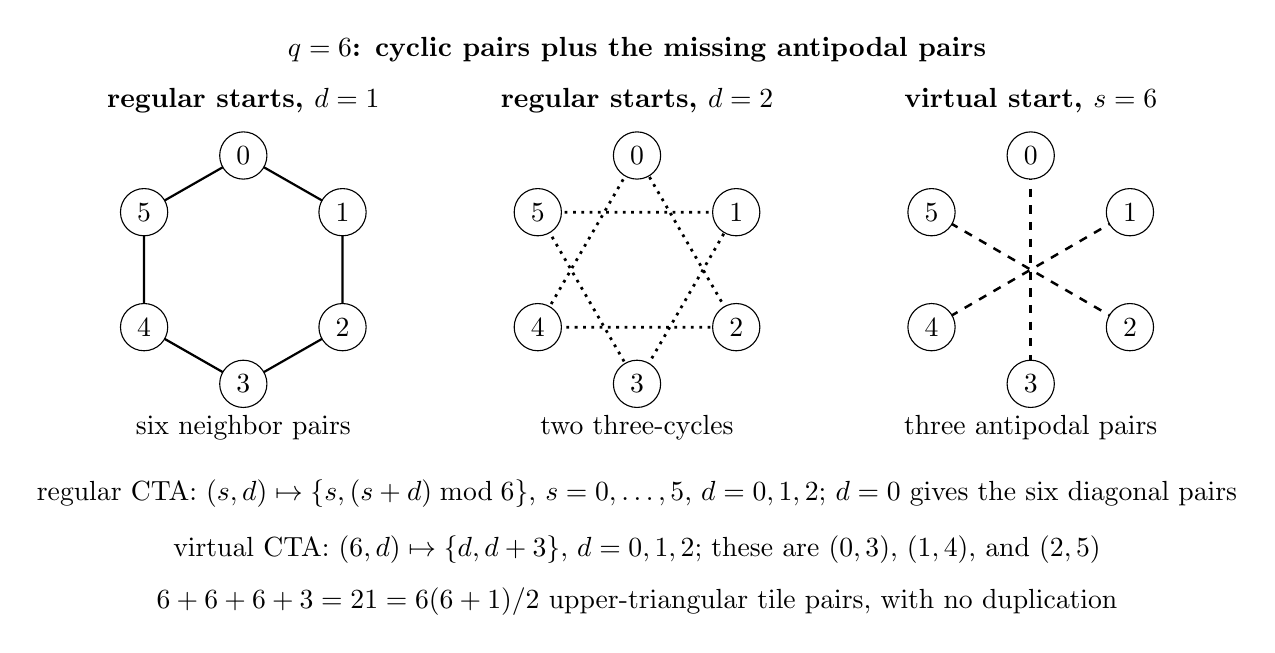
\begin{tikzpicture}
  \node[font=\bfseries] at (5.0,2.8)
    {$q=6$: cyclic pairs plus the missing antipodal pairs};

  \node[font=\bfseries] at (0,2.15) {regular starts, $d=1$};
  \draw[line width=0.8pt] (0,1.45) -- (1.26,0.73) -- (1.26,-0.73) --
    (0,-1.45) -- (-1.26,-0.73) -- (-1.26,0.73) -- cycle;
  \node[draw,circle,fill=white,minimum size=6mm,inner sep=0pt] at (0,1.45) {0};
  \node[draw,circle,fill=white,minimum size=6mm,inner sep=0pt] at (1.26,0.73) {1};
  \node[draw,circle,fill=white,minimum size=6mm,inner sep=0pt] at (1.26,-0.73) {2};
  \node[draw,circle,fill=white,minimum size=6mm,inner sep=0pt] at (0,-1.45) {3};
  \node[draw,circle,fill=white,minimum size=6mm,inner sep=0pt] at (-1.26,-0.73) {4};
  \node[draw,circle,fill=white,minimum size=6mm,inner sep=0pt] at (-1.26,0.73) {5};
  \node at (0,-2.0) {six neighbor pairs};

  \node[font=\bfseries] at (5.0,2.15) {regular starts, $d=2$};
  \draw[dotted,line width=1.0pt] (5.0,1.45) -- (6.26,-0.73) -- (3.74,-0.73) -- cycle;
  \draw[dotted,line width=1.0pt] (6.26,0.73) -- (5.0,-1.45) -- (3.74,0.73) -- cycle;
  \node[draw,circle,fill=white,minimum size=6mm,inner sep=0pt] at (5.0,1.45) {0};
  \node[draw,circle,fill=white,minimum size=6mm,inner sep=0pt] at (6.26,0.73) {1};
  \node[draw,circle,fill=white,minimum size=6mm,inner sep=0pt] at (6.26,-0.73) {2};
  \node[draw,circle,fill=white,minimum size=6mm,inner sep=0pt] at (5.0,-1.45) {3};
  \node[draw,circle,fill=white,minimum size=6mm,inner sep=0pt] at (3.74,-0.73) {4};
  \node[draw,circle,fill=white,minimum size=6mm,inner sep=0pt] at (3.74,0.73) {5};
  \node at (5.0,-2.0) {two three-cycles};

  \node[font=\bfseries] at (10.0,2.15) {virtual start, $s=6$};
  \draw[dashed,line width=0.9pt] (10.0,1.45) -- (10.0,-1.45);
  \draw[dashed,line width=0.9pt] (11.26,0.73) -- (8.74,-0.73);
  \draw[dashed,line width=0.9pt] (11.26,-0.73) -- (8.74,0.73);
  \node[draw,circle,fill=white,minimum size=6mm,inner sep=0pt] at (10.0,1.45) {0};
  \node[draw,circle,fill=white,minimum size=6mm,inner sep=0pt] at (11.26,0.73) {1};
  \node[draw,circle,fill=white,minimum size=6mm,inner sep=0pt] at (11.26,-0.73) {2};
  \node[draw,circle,fill=white,minimum size=6mm,inner sep=0pt] at (10.0,-1.45) {3};
  \node[draw,circle,fill=white,minimum size=6mm,inner sep=0pt] at (8.74,-0.73) {4};
  \node[draw,circle,fill=white,minimum size=6mm,inner sep=0pt] at (8.74,0.73) {5};
  \node at (10.0,-2.0) {three antipodal pairs};

  \node[align=center] at (5.0,-2.85)
    {regular CTA: $(s,d)\mapsto\{s,(s+d)\bmod 6\}$,
     $s=0,\ldots,5$, $d=0,1,2$; $d=0$ gives the six diagonal pairs};
  \node[align=center] at (5.0,-3.55)
    {virtual CTA: $(6,d)\mapsto\{d,d+3\}$,
     $d=0,1,2$; these are $(0,3)$, $(1,4)$, and $(2,5)$};
  \node at (5.0,-4.22)
    {$6+6+6+3=21=6(6+1)/2$ upper-triangular tile pairs, with no duplication};
\end{tikzpicture}
\end{document}
